% !TEX root = ../../handbook-physics.tex
%!TEX TS-program = pdflatex
%!TEX encoding = UTF-8 Unicode


%\documentclass{article}
%\usepackage[svgnames]{xcolor}
%\usepackage{tikz}
%\usepackage{amsmath}
%\usepackage{physics}
%
%\begin{document}
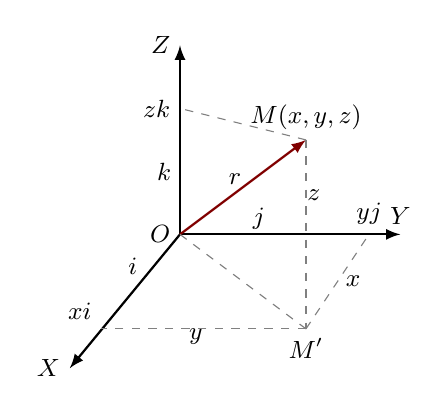
\begin{tikzpicture}[scale=0.4,font=\small]
		\node [] (0) at (0, 6){};
		\node [] (1) at (0, 0) {};
		\node [] (2) at (-3.5, -4.25) {};
		\node [] (3) at (7, 0) {};
		\node [] (4) at (4, 3) {};
		\node [] (5) at (4, -3) {};
		\node [] (6) at (0, 4) {};
		\node [] (7) at (6, 0) {};
		\node [] (8) at (-2.5, -3) {};
		\node [] (9) at (1.75, 1.75) {};
		\node [] (10) at (1.75, 1.75) {$\vb{r}$};
		\node [] (11) at (-0.5, 2) {$\vb{k}$};
		\node [] (12) at (-1.5, -1) {$\vb{i}$};
		\node [] (13) at (2.5, 0.5) {$\vb{j}$};
		\node [] (14) at (0.5, -3.25) {};
		\node [] (15) at (5.5, -1.5) {};
		\node [] (16) at (4.25, 1.25) {};
		\node [] (18) at (5.5, -1.5) {$x$};
		\node [] (19) at (0.5, -3.25) {};
		\node [] (20) at (0.5, -3.25) {$y$};
		\node [] (21) at (4.25, 1.25) {$z$};
		\draw [thick,latex-](0.center) to (1.center);
		\draw [thick,-latex](1.center) to (2.center);
		\draw [thick,-latex](1.center) to (3.center);
		\draw [thick,-latex,Maroon](1.center) to (4.center);
		\draw [dashed,gray](1.center) to (5.center);
		\draw [dashed,gray](4.center) to (6.center);
		\draw [dashed,gray](4.center) to (5.center);
		\draw [dashed,gray](5.center) to (7.center);
		\draw [dashed,gray](5.center) to (8.center);
		\node [left] at (0,0) {$O$};
		\node [left] at (0,6) {$Z$};
		\node [left] at (-3.5, -4.25) {$X$};
		\node [above] at (7, 0) {$Y$};
		\node [above] at (4, 3) {$M (x,y,z)$};
		\node [below] at (4, -3) {$M'$};
		\node [left] at (0,4) {$z\vb{k}$};
		\node [above] at (6,0) {$y\vb{j}$};
		\node [above left] at (-2.5, -3) {$x\vb{i}$};
\end{tikzpicture}
%\end{document}